\section{Résultats}\label{sec-resultats}

\subsection{Métriques globales et rappel par taille}

Le \cref{tab-comparaison} compare les deux modèles sur le jeu de test
(300 images, 2\,551 boîtes de référence). Toutes les métriques globales
progressent : la mAP@0,5 passe de $0{,}438$ à $0{,}825$ ($+88{,}4\,\%$),
la mAP@0,5:0,95 de $0{,}296$ à $0{,}644$ ($+117{,}8\,\%$), la précision
de $0{,}496$ à $0{,}833$ ($+67{,}9\,\%$), le rappel de $0{,}417$ à
$0{,}714$ ($+71{,}1\,\%$) et le F1-score de $0{,}453$ à $0{,}769$
($+69{,}6\,\%$). Le débit d'inférence sur GPU T4 passe de $37{,}2$ à
$43{,}2$ images par seconde ($+16{,}2\,\%$).

\begin{table}[tb]
  \centering
  \caption{Comparaison sur le jeu de test entre YOLOv8n pré-entraîné
  (COCO) et fine-tuné sur le sous-ensemble BMD-45. Le rappel par taille
  suit la convention COCO (petit ${}<32\times32$ px, moyen
  ${}<96\times96$ px, grand au-delà), aires ramenées à la résolution
  d'entrée du réseau (640 px) ; seuil de confiance $0{,}25$,
  $\mathrm{IoU} \geq 0{,}5$. La ligne en gras répond directement à la
  problématique des véhicules éloignés et de petite taille.}
  \label{tab-comparaison}
  \begin{tabular}{lccc}
    \toprule
    Métrique & Pré-entraîné & Fine-tuné & Écart \\
    \midrule
    mAP@0,5          & $0{,}438$ & $0{,}825$ & $+88{,}4\,\%$  \\
    mAP@0,5:0,95     & $0{,}296$ & $0{,}644$ & $+117{,}8\,\%$ \\
    Précision        & $0{,}496$ & $0{,}833$ & $+67{,}9\,\%$  \\
    Rappel           & $0{,}417$ & $0{,}714$ & $+71{,}1\,\%$  \\
    F1-score         & $0{,}453$ & $0{,}769$ & $+69{,}6\,\%$  \\
    Débit (FPS, GPU T4) & $37{,}2$ & $43{,}2$ & $+16{,}2\,\%$ \\
    \midrule
    \textbf{Rappel objets petits} (804 objets)
      & $\mathbf{0{,}122}$ & $\mathbf{0{,}694}$ & $\mathbf{+469{,}4\,\%}$ \\
    Rappel objets moyens (1\,415 objets)
      & $0{,}373$ & $0{,}879$ & $+135{,}6\,\%$ \\
    Rappel objets grands (332 objets)
      & $0{,}792$ & $0{,}952$ & $+20{,}2\,\%$  \\
    \bottomrule
  \end{tabular}
\end{table}

En effectifs, sur les 804 objets petits du jeu de test, le modèle
pré-entraîné en détecte 98 (rappel de $0{,}122$) et le modèle fine-tuné
558 (rappel de $0{,}694$), soit un écart relatif de $+469{,}4\,\%$. Sur
les 1\,415 objets moyens, les détections passent de 528 à 1\,244
($0{,}373$ à $0{,}879$, $+135{,}6\,\%$) ; sur les 332 objets grands, de
263 à 316 ($0{,}792$ à $0{,}952$, $+20{,}2\,\%$). L'écart relatif est
ainsi d'autant plus grand que les objets sont petits :
$+469{,}4\,\%$, $+135{,}6\,\%$ et $+20{,}2\,\%$ pour les trois
catégories de taille. On note que les trois catégories totalisent
$804 + 1\,415 + 332 = 2\,551$ objets, soit exactement le nombre
d'instances du jeu de test (\cref{tab-volumetrie}).

\subsection{Illustrations qualitatives et courbes d'entraînement}

La \cref{fig-demo} montre les détections des deux modèles sur une même
scène d'embouteillage du jeu de test. La \cref{fig-courbes} présente
l'évolution des fonctions de perte et de la mAP sur le jeu de validation
au fil des 50 epochs d'entraînement.

\begin{figure}[tb]
  \centering
  \begin{subfigure}{0.48\linewidth}
    \centering
    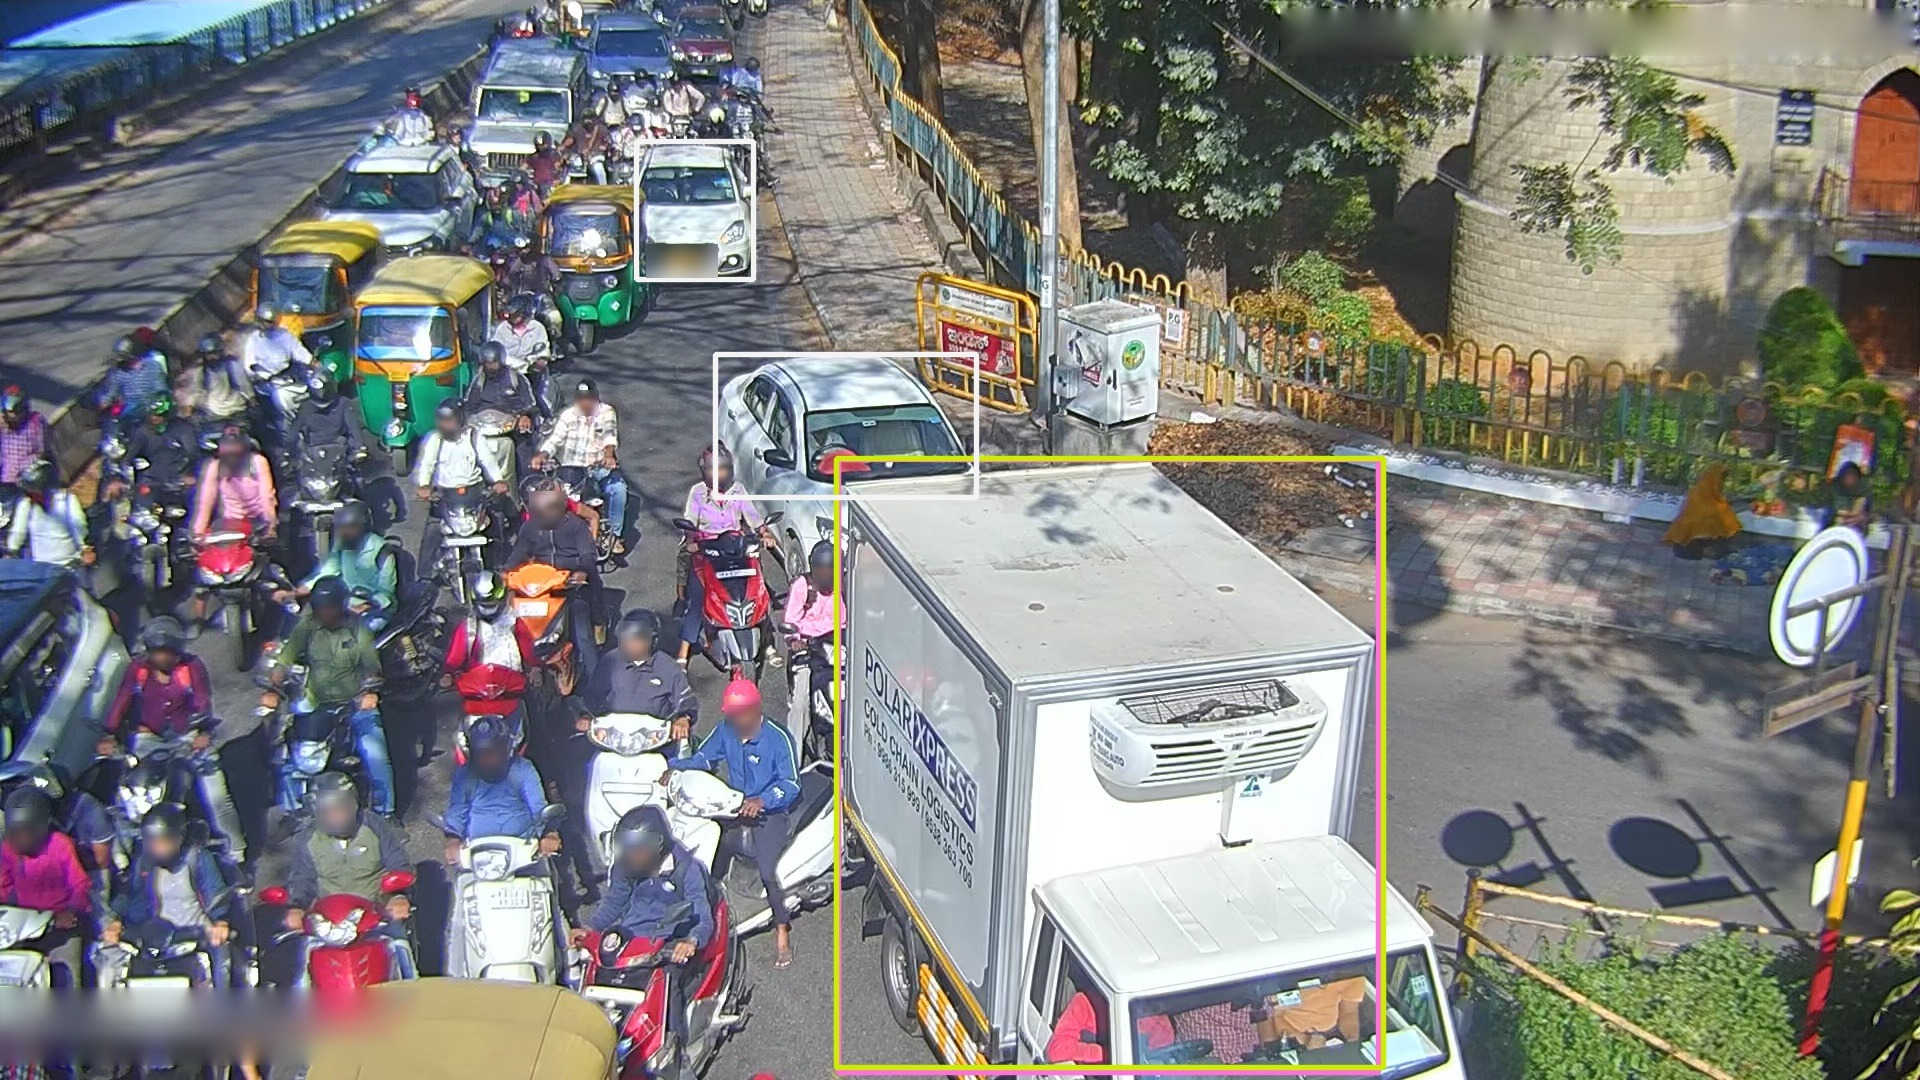
\includegraphics[width=\linewidth]{figures/scene1_base.jpg}
    \caption{YOLOv8n pré-entraîné (COCO) : 4 véhicules détectés.}
    \label{fig-demo-base}
  \end{subfigure}
  \hfill
  \begin{subfigure}{0.48\linewidth}
    \centering
    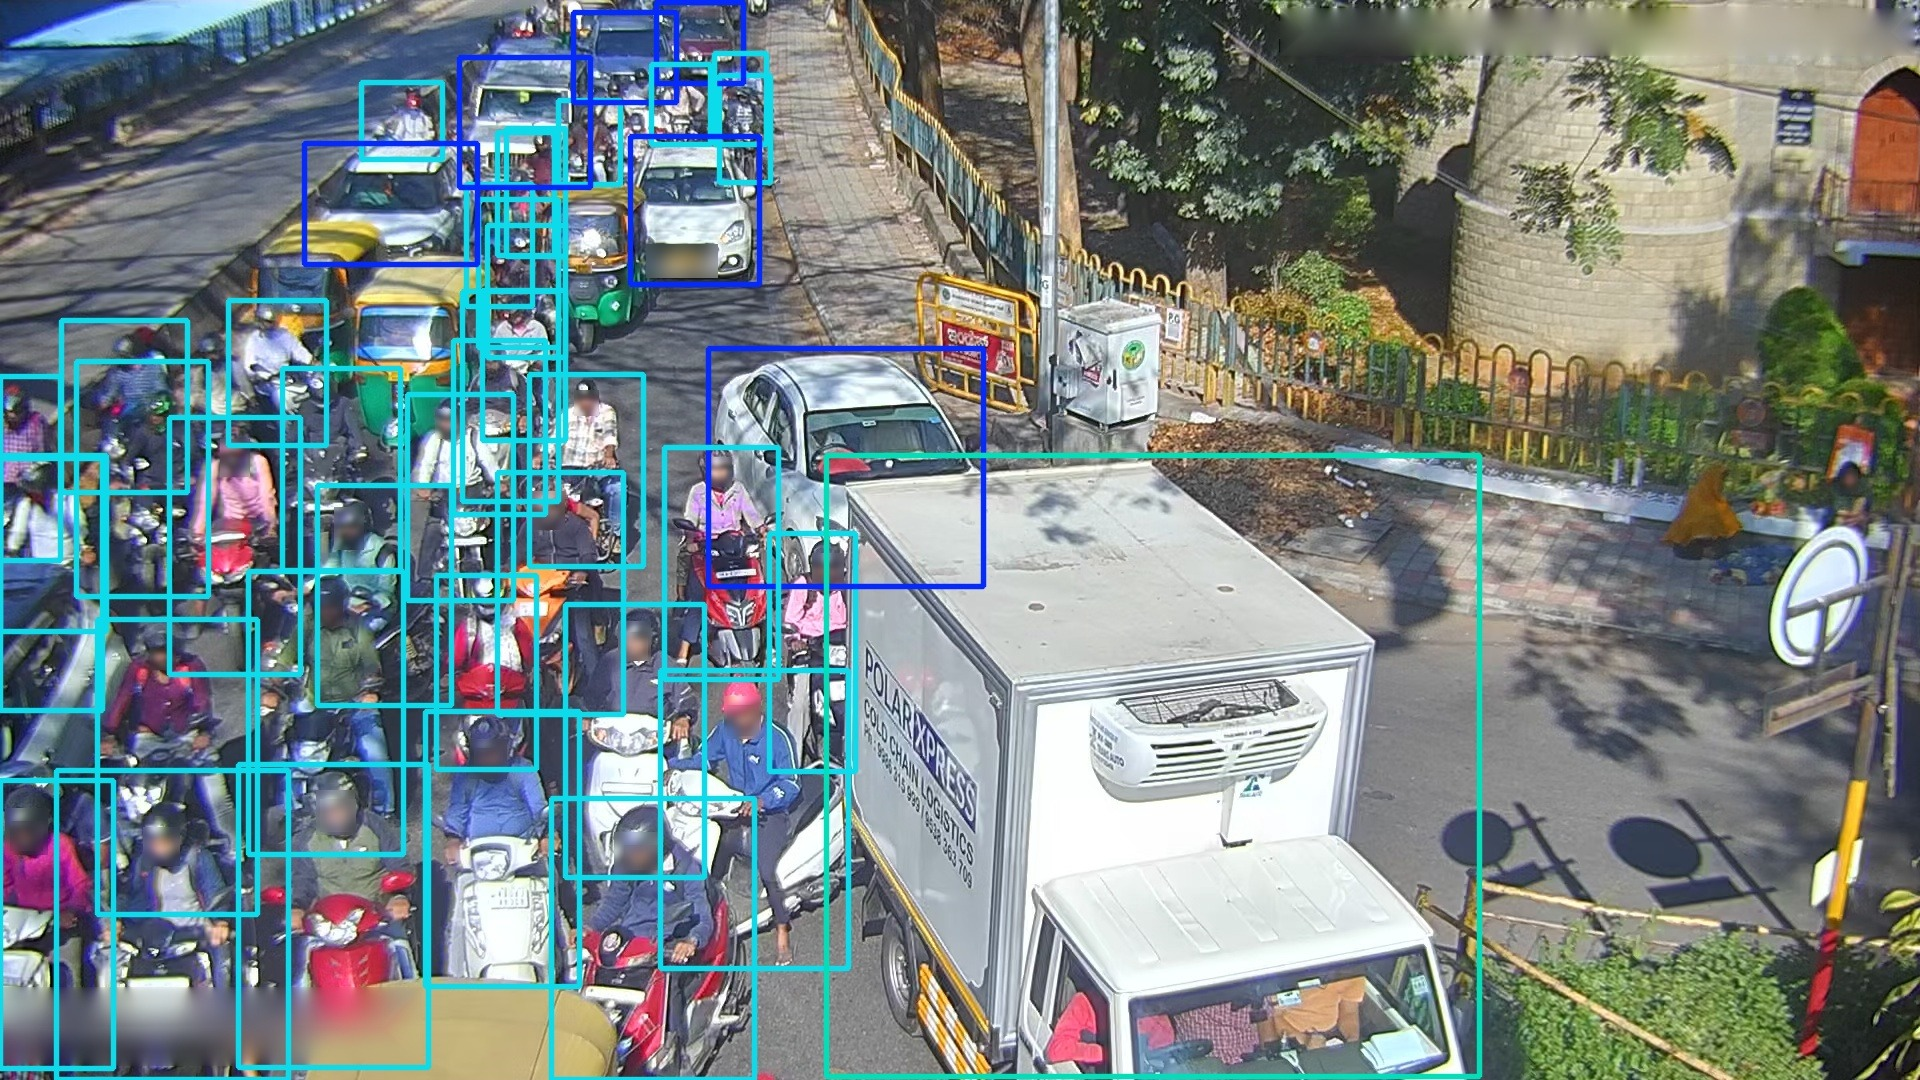
\includegraphics[width=\linewidth]{figures/scene1_finetune.jpg}
    \caption{YOLOv8n fine-tuné : 44 véhicules détectés.}
    \label{fig-demo-finetune}
  \end{subfigure}
  \caption{Détections des deux modèles sur une même scène
  d'embouteillage du jeu de test (image \texttt{val\_000556}, seuil de
  confiance $0{,}25$). Les visages sont floutés à la source dans BMD-45 ;
  la seule plaque d'immatriculation partiellement lisible a été floutée
  par nos soins.}
  \label{fig-demo}
\end{figure}

\begin{figure}[tb]
  \centering
  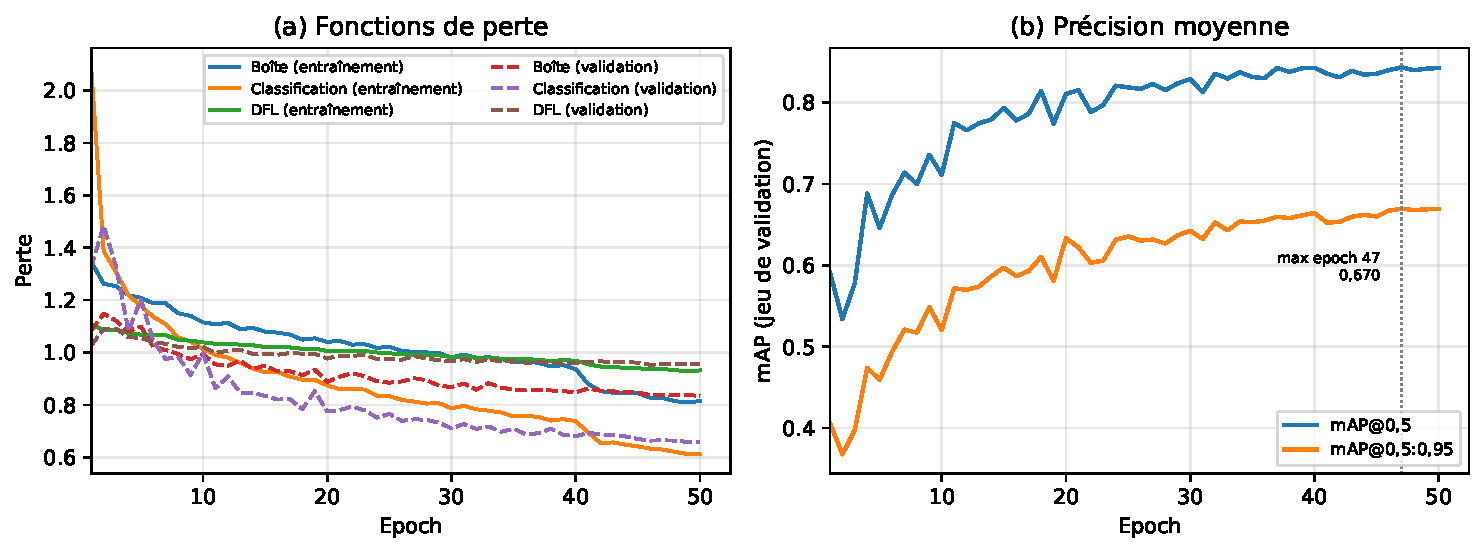
\includegraphics[width=\linewidth]{figures/courbes_entrainement.pdf}
  \caption{Courbes d'entraînement du fine-tuning : fonctions de perte
  (boîte, classification, DFL) et mAP@0,5 et mAP@0,5:0,95 sur le jeu de
  validation, au fil des 50 epochs. Les pertes d'entraînement sont en
  trait plein, celles de validation en pointillés. La ligne verticale
  marque l'epoch 47, où la mAP@0,5:0,95 de validation atteint son
  maximum.}
  \label{fig-courbes}
\end{figure}

\subsection{Dynamique d'entraînement}\label{sec-dynamique}

Les courbes de la \cref{fig-courbes} apportent trois informations que les
métriques finales seules ne donnent pas.

\paragraph{Une convergence rapide puis un plateau.}
La mAP@0,5:0,95 sur le jeu de validation passe de $0{,}406$ après la
première epoch à $0{,}669$ à la cinquantième, avec un maximum de
$0{,}670$ atteint à l'epoch 47. Elle franchit dès l'epoch 29 le seuil de
$95\,\%$ de sa valeur finale : les vingt et une dernières epochs
n'apportent que les $5\,\%$ restants. Le décrochage visible à l'epoch 2,
où la mAP@0,5 recule de $0{,}591$ à $0{,}534$, correspond à la montée en
puissance du taux d'apprentissage pendant la phase d'échauffement, et se
résorbe dès l'epoch 4. L'essentiel de l'adaptation au domaine se joue
donc dans le premier tiers de l'entraînement, ce qui est cohérent avec
l'idée que le fine-tuning réutilise des représentations déjà formées
plutôt qu'il n'en apprend de nouvelles.

\paragraph{Aucun surapprentissage à 50 epochs.}
Les trois pertes d'entraînement décroissent de façon monotone
($1{,}347 \rightarrow 0{,}814$ pour la boîte, $2{,}089 \rightarrow
0{,}611$ pour la classification, $1{,}107 \rightarrow 0{,}932$ pour la
DFL). Surtout, les pertes de validation atteignent leur minimum en toute
fin d'entraînement : epoch 50 pour la perte de boîte, 49 pour la
classification, 46 pour la DFL. L'écart entre pertes d'entraînement et
de validation ne se creuse à aucun moment, et l'arrêt anticipé
(\emph{patience} de 15 epochs, \cref{sec-entrainement}) n'a jamais été
déclenché. Le modèle n'avait donc pas commencé à surapprendre lorsque
l'entraînement s'est arrêté.

\paragraph{Le budget de calcul, et non la convergence, a fixé l'arrêt.}
Les deux observations précédentes se combinent en une conclusion
méthodologique : les 50 epochs constituent une borne que nous avons
imposée, pas un point d'arrêt que les données auraient dicté. Les
métriques rapportées au \cref{tab-comparaison} sont donc à lire comme un
plancher, et non comme le plafond de ce que cette architecture peut
atteindre sur ce jeu. L'entraînement complet a demandé $54{,}9$ minutes
sur GPU T4, ce qui laisse une marge confortable pour prolonger
l'expérience dans le cadre gratuit de Google Colab.
